\documentclass[10pt,a4paper]{scrartcl}

\usepackage[english]{babel}

\input{../Headerfiles/Packages}
\input{../Headerfiles/Titles}
\input{../Headerfiles/Commands}
\graphicspath{{Pictures/}}
\parindent 0pt

\title{System Identification}
\author{
GianAndrea Müller\\
\and
Stefan Rickli
}

\newtheorem{define}{Definition}

%additional commands
\newcommand{\ejon}{(e^{j\omega_n})}
\newcommand{\ejo}{(e^{j\omega})}
\newcommand{\ejzw}{(e^{j(\zeta-\omega_n)})}
\newcommand{\ejz}{(e^{j\zeta})}

\begin{document}
\begin{multicols*}{4}
\maketitle
\tableofcontents
\end{multicols*}

\begin{multicols*}{2}
\section{System Identification}
\section{Definitions}

\begin{define}
A system is said to be \textbf{time invariant} if the response to a certain input is not depending on absolute time.
\end{define}

\begin{define}
A system is said to be \textbf{linear} if its output response to a linear combination of inputs is the same as the linear combination of the output responses of the individual inputs.
\end{define}

\begin{define}
A system is said to be \textbf{causal} if the output at a certain time depends on the input up to that time only.
\end{define}

\begin{define}
A process is said to be \textbf{stationary} if it does not depend on time.
\end{define}

\section{Frequency Domain Methods}

\subsection{Sampling Operation}

\importname{Sampling with period $T$}{$y(k) = \left.y(t)\right|_{t=kT,k=0,1,2,\ldots}$}

\subsection{Fourier Series of Periodic Signals}

\important{$X(e^{j\omega_m})=\sum\limits_{k=0}^{M-1}x(k)e^{-j\omega_m k}$}

\mportant{$\omega_m=\frac{2\pi m}{M}=\omega_0$}

Non-negative frequencies are $m=0$ to $m=M/s$.

They correspond to: $\omega_m = 0,\frac{2\pi}{M},\frac{4\pi}{M},\ldots,\frac{2\pi(M/2-1)}{M},\pi$.

\begin{TDefinitionTable*}
$M$&number of samples&\\
$\omega_0=\frac{2\pi}{M}$&fundamental frequency ($y(k)$)&$\siu{\radian}$\\
$T$&sampling time&$\siu{\second}$\\
$\tau_p=MT$&period&$\siu{\second}$\\
$\omega_0=\frac{2\pi}{\tau_p}$&fundamental frequency ($y(t)$)&$\siu{\radian\per\second}$\\
\end{TDefinitionTable*}

\mportant{$0,\underbrace{\frac{2\pi}{\tau_p}}_{\substack{\text{Fundamental}\\\text{frequency}}},\underbrace{2\left(\frac{2\pi}{\tau_p}\right),\ldots,\frac{M}{2}\left(\frac{2\pi}{\tau_p}\right)}_{\text{Harmonics}}$}

\begin{define}
The highest frequency $\omega_u=\omega_{M/2}=\frac{\pi}{T}$ is called the \textbf{Nyquist frequency}.
\end{define}

\myspic{0.5}{NyquistFrequency}

\begin{TPMatlab}
%Non negative frequency vector
omega = omega_n(N,'p0');
%Discrete Fourier Transform
fft(u); %Matlab
DFT(u); %Lecture
\end{TPMatlab}

\begin{tiny}
Note that the definition of the fft in the Matlab documentation does not describe the actual implementation perfectly. The index actually runs from 0 to $N-1$ as in the definition made in class.
\end{tiny}

\section{Spectral Estimation}

\myspic{0.5}{IODiagram}

\mportname{Transfer function}{$Y(j\omega)=G(j\omega)U(j\omega)$}

\mportname{Discrete time TF}{$Y(e^{j\omega}=G(e^{j\omega}U\ejo$}

\mportant{$\frac{\omega_u}{2\pi}=\frac{r}{NT}$}

\begin{TDefinitionTable*}
$\omega_u$&input frequency&$\siu{\rad\per\second}$\\
$N$&calculation length&$\siu{\ }$\\
$T$&experiment duration?&$\siu{\second}$\\
$r$&some integer&$\siu{\ }$\\
\end{TDefinitionTable*}

\mportname{Input}{$u(k)=\alpha\cos(\omega_u k),\ k=0,1,\ldots,K-1\ \text{ with } K\geq N$}

\mportname{Output}{$y(k)=\alpha\left|G(e^{j\omega_u})\right|\cos(\omega_u k+\theta(\omega_u))+v(k)+\text{transient}$}

where $\theta(\omega_u)=arg(G(e^{j\omega_u})$

\subsection{Sinusoidal correlation methods}

Correlation functions:

\mportant{$I_c(N)=\frac{1}{N}\sum\limits_{k=0}^{N-1}y(k)\cos(\omega_uk)$}

\mportant{$I_s(N)=\frac{1}{N}\sum\limits_{k=0}^{N-1}y(k)\sin(\omega_u k)$}

To calculate those from the data:

\small
\begin{align*}
I_c(N)=\frac{\alpha}{2}\left|G(e^{j\omega_u})\right|\cos(\theta(\omega_u)+\frac{\alpha}{2}\left|G(e^{j\omega_u)}\right|\frac{1}{N}\sum\limits_{k=0}^{N-1}\cos(2\omega_u k+\theta(\omega_u))+\frac{1}{N}\sum\limits_{k=0}^{N-1}v(k)\cos(\omega_u k)
\end{align*}
\normalsize

If the noise, $v(k)$ is sufficiently uncorrelated then the variance satisfies,

\mportant{$\lim\limits_{N\rightarrow\infty}\text{var}\left\{\frac{1}{N}\sum\limits_{k=0}^{N-1}v(k)\cos(\omega_uk)\right\} =0$}

with a convergence rate of $1/N$.

Thus in the limit $N\rightarrow\infty$,

\begin{align*}
E\left\{I_c(N)\right\}&\rightarrow\frac{\alpha}{2}\left|G(e^{j\omega_u})\right|\cos(\theta(\omega_u))\\
E\left\{I_s(N)\right\}&\rightarrow-\frac{\alpha}{2}\left|G(e^{j\omega_u})\right|\sin(\theta(\omega_u))
\end{align*}

and since $\lim\limits_{N\rightarrow\infty}\ \text{var}\left\{I_c(N)\right\}=0,\quad\lim\limits_{N\rightarrow\infty}\ \text{var}\left\{I_s(N)\right\}=0$

The transfer function can be estimated via:

\important{$\hat{G}_N(e^{j\omega_u})=\frac{I_c(N)-jI_s(N)}{\alpha/2}$}

\begin{itemize}
\item Advantages
\begin{itemize}
\item Energy is concentrated at the frequencies of interest.
\item Amplitude of $u(k)$ can easily be tuned as a function of frequency.
\item Easy to avoid saturation and tune signal/noise (S/N) ratio.
\end{itemize}
\item Disadvantages
\begin{itemize}
\item A large amount of data is required.
\item Significant amount of time required for experiments.
\item Some processes won't allow sinusoidal inputs.
\end{itemize}
\end{itemize}

\section{Frequency Domain Methods}

%\textbf{Signals considered}
%
%\begin{itemize}
%\item Finite energy
%\item Periodic
%\item Random
%\item Finite length
%\end{itemize}
%
%\textbf{Signal properties of interest}
%
%\begin{itemize}
%\item Autocorrelation
%\item Crosscorrelation
%\item Frequency domain representation
%\item Spectral density (energy or power)
%\end{itemize}

\mportname{Discrete-time domain signal}{$x(k),\ k=-\infty,\ldots,\infty$}

\importname{Fourier Transform}{$X\ejo=\sum\limits_{k=-\infty}^{\infty}x(k)e^{-j\omega k}$}

\begin{itemize}
\item $X\ejo$ is $2\pi$ periodic.
\item If $\sum\limits_{k=-\infty}^\infty|x(k)|<\infty$ then $X\ejo$ converges.
\end{itemize}

\importname{Inverse Fourier Transform}{$x(k)=\frac{1}{2\pi}\int_{-\pi}^{\pi}X\ejo e^{j\omega k}d\omega$}

where $k=-\infty,\ldots,\infty$

\subsection{Finite Energy Signal}

\subsubsection{Energy Spectral Density (Finite Energy Signal)}

If $x(k)$ is a finite energy signal,

\mportant{$||x(k)||_2^2=\sum\limits_{k=-\infty}^{\infty}|x(k)|^2<\infty$}

\importname{Energy Spectral Density}{$S_x\ejo=|X\ejo|^2$}

\begin{itemize}
\item For finite energy signals the energy spectral density is easily calculated, for signals of infinite length and thus infinite energy however, this is not possible. For that reason the \textbf{power} spectral density is calculated instead!
\end{itemize}

\subsubsection{Autocorrelation (Finite Energy Signal)}

\important{$R_x(\tau)=\sum\limits_{k=-\infty}^{\infty}x(k)x(k-\tau),\quad \tau=-\infty,\ldots,0,\ldots,\infty$}

The spectral density is the Fourier Transform of the autocorrelation:

\mportant{$\sum\limits_{\tau=-\infty}^{\infty}R_x(\tau)e^{-j\omega\tau}=S_x\ejo$}

\begin{TPMatlab}
% autocorrelation for a non-periodic, finite energy signal
Correlation('finen',u); %Lecture
xcorr(u); %Matlab

% crosscorrelation for non-periodic, finite energy signals
Correlation('finen',u,y); %Lecture
xcorr(y,u); %Matlab
\end{TPMatlab}

\subsection{Discrete Periodic Signal}

\mportname{Periodic signal}{$x(k)=x(k+M),\quad \forall\ k\in\{-\infty,\infty\}$}

\mportname{Fundamental frequency}{$\omega_0=\frac{2\pi}{M}$}

\begin{itemize}
\item There are only $M$ unique harmonics of the sinusoid $e^{j\omega_0}$.
\item The non-negative harmonic frequencies are,

\mportant{$e^{jn\omega_0},\ n=0,1,\ldots,M/2$}
\end{itemize}

\begin{TPMatlab}
u_period = sqrt(variance)*randn(N,1)+bias;
u = repmat(u_period,periods,1);
\end{TPMatlab}

\subsubsection{Discrete Fourier Series (Discrete Periodic Signal)}

\important{$X(e^{j\omega_n})=\sum\limits_{k=0}^{N-1}x(k)e^{-j\omega_n k},\ \text{where}\ \omega_n =\frac{2\pi n}{N}=n\omega_0$}

\importname{Inverse Transform}{$x(k)=\frac{1}{N}\sum\limits_{k=0}^{N-1}X(e^{j\omega_n})e^{j\omega_nk}$}

\subsubsection{Autocorrelation (Discrete Periodic Signal)}

\important{$R_x(\tau)=\frac{1}{N}\sum\limits_{k=0}^{N-1}x(k)x(k-\tau)$}

The Fourier transform of $R_x(\tau)$ is now defined as the \textbf{power spectral density}, since it is normalized with the signal length.

\important{$\phi_x(e^{j\omega_n})=\sum\limits_{\tau=0}^{N-1}R_x(\tau)e^{-j\omega_n\tau}=\frac{1}{N}|X(e^{j\omega_n})|^2$}

The energy in a single period is:

\mportant{$\sum\limits_{k=0}^{N-1}|x(k)|^2=\sum\limits_{n=0}^{N-1}\phi_x(e^{j\omega_n})$}

\begin{TPMatlab}
Correlation('periodic',u);
\end{TPMatlab}

\subsubsection{Cross-Correlation (Discrete Periodic Signal)}

\important{$R_{yu}(\tau)=\frac{1}{N}\sum\limits_{k=0}^{N-1}y(k)u(k-\tau)$}

The Fourier transform of $R_{yu}(\tau)$ is now defined as the \textbf{cross-spectral density}.

\important{$\phi_{yu}(e^{j\omega_n})=\sum\limits_{\tau = 0}^{N-1}R_{yu}(\tau)e^{-j\omega_n\tau}) = \frac{1}{N}Y(e^{j\omega_n})U^\ast(e^{j\omega_n})$}

\begin{TPMatlab}
Correlation('periodic',u,y);
\end{TPMatlab}

\subsection{Random Signal}

Normally distributed noise:

\important{$e(k)\in\mathcal{N}(0,\lambda)\Rightarrow\begin{cases}\expe{e(k)}=0\text{ (zero mean)}\\\expe{|e(k)|^2}=\lambda\text{ (variance)}\end{cases}$}

The $e(k)$ are independent and identically distributed (i.i.d.).

\begin{TPMatlab}
standard_deviation = 2;
variance = standard_deviation^2;
bias = 0;
N = 1024;
u = randn(N,1)*standard_deviation + bias;
\end{TPMatlab}

\subsubsection{Autocovariance (Random Signal)}

\begin{align*}
R_x(\tau) &= \expe{x(k)x(k-\tau)}\\
&=\expe{x(k)x^\ast(k-\tau)} \text{ (in the complex case)}\\
&=\expe{x(k)x^\ast(x-\tau)} \text{ (in the multivariable case)}
\end{align*}

General (non-stationary, non-zero mean) case:

\begin{align*}
R_x(s,t)&=\expe{(x(s)-\expe{x})(x(t)-\expe{E})}\\
&= \expe{x(s)x(t)}\text{ (if zero mean)}\\
&= R_x(s-t)\text{ (if stationary)}
\end{align*}

Further properties are

\begin{itemize}
\item $R_x(-\tau)=R_x^\ast(\tau)$
\item $R_x(0)\geq |R_x(\tau)|\ \forall\tau>0$
\end{itemize}

\begin{TPMatlab}
xcorr(u)/N; %Lecture 3.37
\end{TPMatlab}

\subsubsection{Power Spectral Density (Random Signal)}

\important{$\phi_x\ejo:=\sum\limits_{\tau=-\infty}^{\infty}R_x(\tau)e^{-j\omega\tau}$ where $\omega\in[-\pi,\pi)$}

For a zero-mean random signal:

\mportant{$\lim\limits_{N\rightarrow\infty}\frac{1}{N}\sum\limits_{k=0}^{N-1}|x(k)|^2=\var{x(k)}=\frac{1}{2\pi}\int_{-\pi}^{\pi}\phi_x\ejo d\omega$}


Further properties are

\begin{itemize}
\item $\phi_x\ejo\in\mathbb{R}$
\item $\phi_x\ejo\geq 0\ \forall\ \omega$
\item $\phi_x\ejo=\phi_x(e^{-j\omega})$ for all real-valued $x(k)$
\end{itemize}

\begin{TPMatlab}
fft(xcorr(u)/N)) %Lecture 3.37 (?)
\end{TPMatlab}

\subsubsection{Cross-Covariance (Random Signal)}

\important{$R_{yu}(\tau)=\expe{(y(k)-\expe{y(k)})(u(k-\tau)-\expe{u(k)}}$}

For zero mean signals:

\mportant{$R_{yu}(\tau)=\expe{y(k)u(k-\tau)}$}

Joint stationarity is required to make the definition dependent on $\tau$ only.

If $R_{yu}(\tau)=0$ for all $\tau$ then $y(k)$ and $u(k)$ are uncorrelated.

\begin{TPMatlab}
xcorr(u,y)/N; %Lecture 3.37 (?)
\end{TPMatlab}

\subsubsection{Cross Power Spectral Density (Random Signal)}

\important{$\phi_{yu}\ejo=\sum\limits_{\tau=-\infty}^\infty R_{yu}(\tau)e^{-j\omega\tau},\ \omega\in[-\pi,\pi)$}

The inverse is,

\mportant{$R_{yu}(\tau)=\frac{1}{2\pi}\int_{-\pi}^\pi\phi_{yu}\ejo e^{j\omega\tau}d\omega$}

\begin{TPMatlab}
fft(xcorr(y,u)/N); %Lecture 3.37 (?)
\end{TPMatlab}

\subsection{Finite Length Signal}

\subsubsection{Discrete-Fourier Transform (Finite Length Signal)}

\important{$X_N(e^{j\omega_n})=\sum\limits_{k=0}^{N-1}x(k)e^{-j\omega_nk},$ where $\omega_n=\frac{2\pi n}{N}$}

The inverse DFT is

\mportant{$x(k)=\frac{1}{N}\sum\limits_{n=0}^{N-1}X_N(e^{j\omega_n})e^{j\omega_n k},\quad k=0,\ldots, N-1$}

\subsubsection{Periodogram (Finite Length Signal)}

\important{$\frac{1}{N}\left|V_N\ejo\right|^2$}

An asymptotically unbiased estimator of the spectrum is

\mportant{$\lim\limits_{N\rightarrow\infty}\expe{\frac{1}{N}|V_N(e^{j\omega}|^2}=\phi_v(\omega)$}

This assumes that the autocorrelation decays quickly enough:

\mportant{$\lim\limits_{N\rightarrow\infty}\frac{1}{N}\sum\limits_{\tau=-N}^N|\tau R_v(\tau)| =0$}

\section{ETFE}

\myspic{0.5}{IODiagram}

Linear, time-invariant system, $g(l)$:

\mportant{$y(k)=\sum\limits_{l=0}^\infty g(l)u(k-l)+v(k),\quad k=0,1,\ldots$}

Assumptions:

\begin{enumerate}
\item causal system: $g(l) = 0,\forall l<0$
\item noise: $E\{v(k)\} = 0$, zero mean, stationary
\end{enumerate}

Given $\{u(k),y(k)\}$ find an estimate $\hat{G}\ejo$ such that it fits the $G\ejo$.

\importname{Bias}{Bias($\hat{G}))G-E\{\hat{G}\}$}

\importname{Variance}{var($(\hat{G})=E\left\{|\hat{G}-E\{\hat{G}\}|^2\right\}$}

\importname{Mean-square error}{MSE$(\hat{G})=E\left\{|G-\hat{G}|^2\right\}$}

Note that MSE$(\hat{G})=$var$(\hat{G})+$Bias$^2(\hat{G})$.

\subsection{Input-output relationship}

For finite energy signals:

\mportant{$y(k) = \sum\limits_{l=0}^\infty g(l)u(k-l)+v(k)$}

\mportant{$Y\ejo=G\ejo U\ejo+V\ejo$}

which in the idealized case leads to:

\important{$\frac{Y\ejo}{U\ejo}=G\ejo+\frac{V(e^j\omega)}{U\ejo}\approx G\ejo$}

In reality we only have $N$ samples:

\mportant{$\underbrace{Y_N(e^{j\omega_n})}_{\text{length-N DFT}} = \sum\limits_{k=0}^{N-1}y(k) e^{-j\omega_n k}\approx \sum\limits_{k=-\infty}^\infty y(k)e^{-j\omega_n k}=Y(e^{j\omega_n}$}

\mportant{$\underbrace{U_N(e^{j\omega_n})}_{\text{length-N DFT}}=\sum\limits_{k=0}^{N-1}u(k)e^{-j\omega_n k}\approx \sum\limits_{k=-\infty}^\infty u(k)e^{-j\omega_n k}=U(e^{j\omega_n})$}

\importname{ETFE}{$\hat{G}_N(e^{j\omega_n}):=\frac{Y_N(e^{j\omega_n})}{U_N(e^{j\omega_n})}$}

\subsection{Periodic input case}

Period $M$ inputs: $u(k)=u(k+M)$

If $sM = N$ for an integer $s$, the fourier series over N samples is equal to the real fourier series!

\mportant{$U_N(e^{j\omega_n}) = U(e^{j\omega_n})\forall \omega_n=\frac{2\pi n}{N},\ n=0,\ldots,N-1$}

Then

\mportant{$Y_N(e^{j\omega_n})=G(e^{j\omega_n})U_N(e^{j\omega_n})+V_N(e^{j\omega_n})$}

\mportant{$\hat{G}_N(e^{j\omega_n})=G(e^{j\omega_n})+\frac{V_N(e^{j\omega_n})}{U_N(e^{j\omega_n})}$}

%\subsubsection{Error properties}

\textbf{Bias:}

\mportant{$E\{\hat{G}_N(e^{j\omega_n})\}=G(e^{j\omega_n})+E\left\{\frac{V_N(e^{j\omega_n})}{U_N(e^{j\omega_n})}\right\}=G(e^{j\omega_n})$}

when assuming zero mean noise. Thus for periodic inputs with $N$ being an integer number of periods, \textbf{the ETFE is unbiased}.

\textbf{Variance:}

For the unbiased case:

\renewcommand{\expe}[1]{\text{E}\left\{#1\right\}}

\mportant{$E\left\{|\hat{G}_N(e^{j\omega_n})-G(e^{j\omega_n})|^2\right\}=\frac{\phi_v(e^{j\omega_n})+\frac{2}{N}c}{\frac{1}{N}|U_N(e^{j\omega_n})|^2}$}

where $|c|\leq C=\sum\limits_{\tau =1}^\infty |\tau R_v(\tau)|$ is assumed to be finite.

For estimates at different frequencies ($\omega_n\neq\omega_i$):

\mportant{$E\left\{(\hat{G}_N(e^{j\omega_n})-G(e^{j\omega_n}))(\hat{G}_N(e^{-j\omega_i)}-G(e^{-j\omega_i}))\right\}=0$}

\textbf{Transient responses:}

Initial transient corrupts the measurement

\mportant{$y(k)=G(u_{periodic}(k)W_{[0,N-1]}(k))+v(k)$}

with the window function:

\mportant{$W_{[0,N-1]}(k)=\begin{cases}
1&\text{ if } 0\leq0<N\\
0&\text{ otherwise}\end{cases}$}

For all outputs up to time $k=N-1$

\mportant{$y(k)=Gu_{periodic}(k)-\underbrace{G(u_{periodic}W_{(-\infty,-1)})}_{r(k)}+v(k)$}

\mportant{$Y_N(e^{j\omega_n})=G(e^{j\omega_n})U_N(e^{j\omega_n})+R_N(e^{j\omega_n})+V_N(e^{j\omega_n})$}

The input in negative time, which is present in a ideal periodic input, and missing in a real periodic input, has an influence on positive time, which is described by $r(k)$.

\vspace{3ex}

When using a periodic signal multiple times the resulting DFT does not contain more information, since in a periodic signal there are only a certain number of frequencies contained, but the energy in those frequencies increases!

\textbf{Transient bias error:}

\mportant{$\hat{G}\ejon=\frac{Y_N\ejon}{U_N\ejon}=G\ejon+\frac{R_N\ejon}{U_N\ejon}+\frac{V_N\ejon}{U_N\ejon}$}

\textbf{For periodic $u(k)$}

As $N=mM,m\rightarrow\infty$

\mportant{$|U_N\ejon|=m|U_M\ejon|$}

\textbf{For random $u(k)$}

As $N\rightarrow\infty$

\mportant{$E\{|U_N\ejon|\}\rightarrow\sqrt{N}\sqrt{\phi_u\ejon}$}

Thus

\important{$\left|\frac{R_N\ejon}{U_N\ejon}\right|\rightarrow 0$ with rate $\begin{cases}
\frac{1}{N}&\text{ for periodic input}\\
\frac{1}{\sqrt{N}}&\text{ for random inputs}\end{cases}$}

A fix for getting rid of the influence of the transient response: Get rid of the first period.

\begin{TPMatlab}
r = 4;
N_split = N/r;
u_re = reshape(u(N_split+1:end),N_split,[]);
y_re = reshape(y(N_split+1:end),N_split,[]);

U_re = fft(u_re);
Y_re = fft(y_re);

G_re = Y_re./U_re;

G_avg = mean(G_re,2);
\end{TPMatlab}

\subsection{Spectral Transformations}

If $v(k) = 0$

\mportant{$\phi_y\ejon=G\ejon\phi_u\ejon G^T\ejon$}

where $G^T\ejon$ is the complex conjugate of $G\ejon$.

If $v(k)\neq 0$ and uncorrelated

\mportant{$\phi_y\ejon = |G\ejon|^2\phi_u\ejon+|H\ejon|^2$}

But this approach has no more phase information. For that reason use the cross spectrum:

\mportant{$\phi_{yu}\ejon=G\ejon\phi_u\ejon+\phi_{uv}\ejon = G\ejon\phi_u\ejon$}

if $u(k)$ and $v(k)$ are uncorrelated.

\importname{Spectral estimation methods}{$\hat{G}\ejo = \frac{\hat{\phi}_{yu}\ejon}{\hat{\phi}_u\ejon}$}

where

\mportant{$\phi_y\ejon=|G\ejon|^2\phi_u\ejon+\phi_v\ejon$}

\mportant{$\phi_{yu}\ejon=G\ejon\phi_u\ejon$}

\subsection{Approaches to spectral estimation}

\subsubsection{Spectral estimation (Periodogram)}

The periodogram is an asymptotically unbiased estimator of the spectrum given $\lim\limits_{n\rightarrow\infty}\frac{1}{N}\sum\limits_{\tau=-\N}^N|\tau R_v(\tau)|=0$

\mportname{Periodogram}{$\frac{1}{N}|V_N\ejon|^2$}

\important{$\lim\limits_{N\rightarrow\infty}E\left\{\frac{1}{N}|V_N\ejon|^2\right\}=\phi_v\ejon$}

which is under the assumption

\mportant{$\lim\limits_{N\rightarrow\infty}\frac{1}{N}\sum\limits_{\tau=-N}^{N}|\tau R_v(\tau)|=0$}

\subsubsection{Spectral estimation (via covariances)}
\label{sec:SpectralEstimationCovariance}

The autocovariance of the noise for stochastic $v(k)$ is described as:

\mportant{$\hat{R}_v(\tau)=\begin{cases}
\frac{1}{N-|\tau|}\sum\limits_{k=\tau}^{N_1}v(k)v(k-\tau),&\text{for }\tau\geq 0\\
\frac{1}{N-|\tau|}\sum\limits_{k=0}^{N+\tau-1}v(k)v(k-\tau),&\text{for }\tau<0
\end{cases}$}

This is an unbiased estimator of $R_v(\tau)$: $\expe{\hat{R}_v(\tau)}=R_v(\tau)$

\important{$\hat{\phi}_v\ejon=\sum\limits_{\tau=-N+1}^{N-1}\hat{R}_v(\tau)e^{-j\omega \tau}$}

\begin{TPMatlab}
xcorr(a-mean(a))-xcov(a) == 0 %true
\end{TPMatlab}

The functions above both calculate the zero-mean shifted autocorrelation of a signal which is \textbf{not} equivalent to the autocovariance of the signal! They lack the normalization by $N-|\tau|$!

\begin{TPMatlab}
Covariance('zero-mean',a);
Covariance('zero-mean',a,b);
\end{TPMatlab}

\subsubsection{Spectral estimation (periodic signals)}

Periodic signal $x(k)$ with period $M$, $N=mM$ for some integer $m$

\mportant{$R_x(\tau)=\frac{1}{M}\sum\limits_{k=0}^{M-1}x(k)x(k-\tau)$}

The power spectral density can be calculated and is equal to the periodogram:

\important{$\phi_x\ejon=\sum\limits_{\tau = 0}^{M-1}R_x(\tau)e^{-j\omega_n\tau}=\frac{1}{M}\left|X_M\ejon\right|^2$}

\begin{TPMatlab}
Ru = Correlation('periodic',u);
\end{TPMatlab}

\subsubsection{Spectral estimation (more general case)}

Alternative autocorrelation estimate:

\mportant{$\hat{R}_x(\tau)=\begin{cases}
\frac{1}{N}\sum\limits_{k=\tau}^{N-1}x(k)x(k-\tau),&\text{ for }\tau\geq 0\\
\frac{1}{N}\sum\limits_{k=0}^{N+\tau-1}x(k)x(k-\tau),&\text{ for }\tau<0\end{cases}$}

Periodic $x(k)$: unbiased (exact) if $N=mM$

\vspace{3ex}

Random $x(k)$ biased $\expe{\hat{R}_x(\tau)}=\frac{N-|\tau|}{N}R_x(\tau)$.

asymptotically biased as $N\rightarrow\infty,\tau/N\rightarrow 0$

\begin{TPMatlab}
Ru = xcorr(u)/N;
\end{TPMatlab}

\begin{itemize}
\item The bias when estimating $R_x$ for a random signal has the form a triangular weighting across $\tau$. A scaling of the signal would remove the bias, which is effectively done by the spectral estimation for via covariances \ref{sec:SpectralEstimationCovariance}.
\end{itemize}

\section{Averaging and Smoothing}

Multiple experiments $u_r(k),y_r(k), r=1\ldots,R, k=0,\ldots, K-1$

\mportant{$\hat{G}\ejon=\sum\limits_{r=1}^R\alpha_r\hat{G}_r\ejon$}

where $\sum\limits_{r=1}^G\alpha_r = 1$ and for calculating the average $\alpha_r =\frac{1}{R}$.

\vspace{3ex}

The averaging can be optimized by selecting $\alpha_r$ such that the variance $\sigma_r^2\ejon$ is minimized.

\mportant{$\var{\hat{G}\ejon}=\var{\sum\limits_{r=1}^R\alpha_r\ejon \hat{G}_r\ejon}=\sum\limits_{r=1}^R\alpha_r^2\sigma_r^2\ejon$}

This is minimized by

\important{$\alpha_r\ejon=\frac{1/\sigma_r^2\ejon}{\sum\limits_{r=1}^T1/\sigma_r^2\ejon}$}

Thus the signal is weighted inversely proportional to the variance.

\vspace{3ex}

Thus if $\var{\hat{G}_r\ejon}=\frac{\phi_v\ejon}{\frac{1}{N}|U_r\ejon|^2}$ then $\alpha_r\ejon=\frac{|U_r\ejon|^2}{\sum\limits_{r=1}^R|U_r\ejon|^2}$.

\vspace{3ex}

The best result is obtained if the input is the same for all $r$, which will lead to a reduction of the variance as follows:

\mportant{$\var{\hat{G}\ejon}=\frac{\var{\hat{G}_r\ejon}}{R}$}

Biased estimates will reduce the improvement in variance.

\begin{itemize}
\item Since we are adding complex numbers the magnitude of the average is not equal to the average of the magnitudes $r_i$.
\end{itemize}

\subsection{Bias-variance trade-offs in data record splitting}

Divide a data record into smaller parts for averaging:

\mportant{$\{u(k),y(k)\}, k=0,\ldots,K-1$}

Choose $R$ records and calculation length $N$, such that $NR\leq K$:

\mportant{$u_r(n) = u(rN+n)$}

And average the resulting estimates:

\important{$\hat{G}\ejon=\frac{1}{R}\sum\limits_{r=0}^{R-1}\hat{G}_r\ejon=\frac{1}{R}\sum\limits_{r=0}^{R-1}\frac{\hat{Y}_r\ejon}{\hat{U}_r\ejon}$}

As $R$ increases:
\begin{itemize}
\item The number of points calculated, $N$ decreases.
\item The variance decreases (by up to $1/R$).
\item The bias increases (due to non-periodicity transients).
\end{itemize}

Mean-square error
\begin{itemize}
\item Transient bias grows linearly with the number of data splits.
\item Variance decays with a rate of up to $1/$(number of averages).
\end{itemize}

What if there is no option of running periodic input experiments? $\rightarrow$ exploit the assumed smoothness of the underlying system.

\subsection{Smoothing the ETFE}

Assume the true system to be close to constant for a range of frequencies: $G(e^{j\omega_{n+r}})\approx G(e^{j\omega_n})$ for $r=0,\pm 1,\ldots,\pm r$.

The minimum variance smoothed estimate is:

\mportant{$\tilde{G}_N\ejon=\frac{\sum\limits_{r=-R}^R\alpha_r\hat{G}_N(e^{j\omega_{n+r}})}{\sum\limits_{r=-R}^R\alpha_r},\qquad \alpha_r=\frac{\frac{1}{N}|U_N(e^{j\omega_{r+n}})|^2}{\phi_v(e^{j\omega_{n+r}})}$}

The summation above can then be approximated by an integral:

\mportant{$\approx \frac{\int_{\omega_{n-r}}^{\omega_{n+r}}\alpha\ejz\hat{G}_N\ejz d\zeta}{\int_{\omega_{n-r}}^{\omega_{n+r}}\alpha\ejz d\zeta},\qquad \text{with } \alpha\ejz=\frac{\frac{1}{N}|U_N\ejz|^2}{\phi_v\ejz}$}

Which can be reformulated using a smoothing window:

\mportant{$\tilde{G}_N\ejon=\frac{\frac{1}{2\pi}\int_{-\pi}^\pi W_\gamma\ejzw\alpha\ejz\hat{G}_N\ejz d\zeta}{\frac{1}{2\pi}\int_{-\pi}^\pi W_\gamma\ejzw\alpha\ejz d\zeta}\qquad\text{with }\alpha\ejz=\frac{\frac{1}{N}|U_N\ejz|^2}{\phi_v\ejz}$}

\subsubsection{Assumptions on $\phi_v\ejo$}

Assume $\phi_v\ejo$ is also a smooth function of frequency.

\mportant{$\frac{1}{2\pi}\int_{-\pi}^\pi W_\gamma\ejzw\left|\frac{1}{\phi_v\ejz}-\frac{1}{\phi\ejon}\right| d\zeta\approx 0$}

Then use,

\mportant{$\alpha\ejz=\frac{\frac{1}{N}|U_N\ejz|^2}{\phi_v\ejon}$}

to get

\important{$\tilde{G}_N\ejon=\frac{\frac{1}{2\pi}\int_{-pi}^\pi W_\gamma(e^{-j(\zeta-\omega_n)})\frac{1}{N}|U_N\ejz|^2\hat{G}_N\ejz d\zeta}{\frac{1}{2\pi}\int_{-\pi}^\pi W_\gamma\ejzw\frac{1}{N}|U_N\ejz^2d\zeta}$}

The wider the frequency window (decreasing $\gamma$)

\begin{itemize}
\item the more adjacent frequencies included in the smoothness estimate.
\item the smoother the result.
\item the lower the noise induced variance.
\item the higher the bias.
\end{itemize}

\subsubsection{Characteristic windows}

\importname{Bartlett}{$W_\gamma\ejo=\frac{1}{\gamma}\left(\frac{\sin\gamma\omega/2}{\sin\omega/2}\right)^2$}

\importname{Hann}{$W_\gamma\ejo=\frac{1}{2}D_\gamma(\omega)+\frac{1}{4}D_\gamma(\omega-\pi/\gamma)+\frac{1}{4}D_\gamma(\omega+\pi/\gamma)$}

where 

\mportant{$D_\gamma(\omega)=\frac{\sin\omega(\gamma+0.5)}{\sin\omega/2}$}

\textbf{Properties of window functions:}

\begin{itemize}
\item $\frac{1}{2\pi}\int_{-\pi}^\pi W_\gamma\ejz d\zeta=1$
\item $\int_{-\pi}^\pi\zeta W_\gamma\ejz d\zeta=0$
\item $M(\gamma):=\int_{-\pi}^\pi\zeta^2W_\gamma\ejz d\zeta$
\item $\bar{W}(\gamma):=2\pi\int_{-\pi}^\pi W_\gamma^2\ejz d\zeta$
\end{itemize}

\begin{tabular}{lll}
Bartlett&$M(\gamma)=\frac{2.78}{\gamma},$&$\bar{W}(\gamma)\approx 0.67\gamma\quad$(for $\gamma>5$)\\
Hamming&$M(\gamma)=\frac{\pi^2}{2\gamma^2},$&$\bar{W}(\gamma)\approx 0.75\gamma\quad$(for $\gamma>5$)
\end{tabular}

\begin{itemize}
\item $M(\gamma)$ gives an idea of the bias effect.
\item $\bar{W}(\gamma)$ gives an idea of the variance effect.
\end{itemize}

\subsubsection{Asymptotic bias properties}

\mportant{$\expe{\tilde{G}\ejon-\expe{G\ejon}}=\expe{\tilde{G}\ejon-G\ejon}=M(\gamma)\left(\frac{1}{2}\underbrace{G''\ejon}_\text{curvature}+\underbrace{G'\ejon}_{slope}\frac{\phi_u'\ejon}{\phi_u\ejon}\right)+H.O.T.$}

Increasing $\gamma$

\begin{itemize}
\item makes the frequency window smaller.
\item averages over fewer frequency values.
\item makes $M(\gamma)$ smaller
\item reduces the bias of the smoothed estimate $\tilde{G}\ejon$
\end{itemize}

\subsubsection{Asymptotic variance properties}

\mportant{$\expe{(\tilde{G}\ejon-\expe{\tilde{G}\ejon})^2}=\frac{1}{N}\bar{W}(\gamma)\frac{\phi_v\ejon}{\phi_u\ejon}+H.O.T.$}

Increasing $\gamma$

\begin{itemize}
\item makes the frequency window narrower.
\item averages over fewer frequency values.
\item makes $\bar{W}_\gamma$ larger.
\item increases the variance of the smoothed estimate $\tilde{G}\ejon$.
\end{itemize}

\subsubsection{Asymptotic MSE properties}

\mportant{$\expe{|\tilde{G}\ejon-G\ejon|^2}\approx M^2(\gamma)|F\ejon|^2+\frac{1}{N}\bar{W}(\gamma)\frac{\phi_v\ejon}{\phi_u\ejon}$}

where 

\mportant{$F\ejon=\frac{1}{2}G''\ejon+G'\ejon\frac{\phi'_u\ejon}{\phi_u\ejon}$}

If $M(\gamma)=M/\gamma^2$ and $\bar{W}(\gamma)=\bar{W}\gamma$ then MSE is minised by:

\important{$\gamma_{optimal}=\left(\frac{4M^2|F\ejon|^2\phi_u\ejon}{\bar{W}\phi_v\ejon}\right)^{1/5}N^{1/5}$}

and 

\mportant{MSE at $\gamma_{optimal}\approx CN^{-4/5}$}

\section{Windowing and Input Signals}

\mportant{$\phi_{yu}\ejo=G\ejo\phi_u\ejo$}

\important{$\hat{G}\ejon=\frac{\hat{\phi}_{yu}\ejon}{\hat{\phi}_u\ejon}$}

Recall that the smoothed ETFE is:

\mportant{$\tilde{G}_N\ejon=\frac{\frac{1}{2\pi}\int_{-\pi}^\pi W_\gamma\ejzw\frac{1}{N}|U_N\ejz|^2\hat{G}_N\ejz d\zeta}{\frac{1}{2\pi}\int_{-\pi}^\pi W_\gamma \ejzw\frac{1}{N}|U_n\ejz|^2d\zeta}$}

The denominator term approaches $\frac{1}{2\pi}\int_{-\pi}^\pi W_\gamma\ejzw \phi\ejon d\zeta$ as $N\rightarrow \infty$. 

\vspace{3ex}

If in addition $W_\gamma\ejo$ is concentrated around $\zeta = 0$ (i.e. $\gamma/N\rightarrow 0$) then the denominator term approaches $\phi_u\ejon$ as $N\rightarrow\infty$.

\vspace{3ex}

This motivates the smoothed spectral estimate:

\important{$\tilde{\phi}_u\ejon=\frac{1}{2\pi}\int_{-\pi}^\pi W_\gamma\ejzw\frac{1}{N}|U_N\ejo|^2d\zeta$}

Similarly the numerator approaches $\phi_{yu}$ as $N\rightarrow\infty$:

\important{$\tilde{\phi}_{yu}\ejon=\frac{1}{2\pi}\int_{-\pi}^\pi W_\gamma\ejzw\frac{1}{N}|U_N\ejo|^2\hat{G}_N\ejo d\zeta$}

For this reason the smoothed ETFE is equal to the smoothed spectral estimate for $N\rightarrow \infty$.

\subsection{Frequency domain smoothing in matlab}

\begin{TPMatlab}
gamma = 80;
U = fft(u); Y = fft(y);
G_est = Y./U;
G_est_smooth = G_est*0;

[om,Wg] = WfHann(g,N);
%shift to start at zero
zidx = find(om == 0);
omega = [om(zidx:N);om(1:zidx-1)];
Wg = [Wg(zidx:N) Wg(1:zidx-1)];
%variance weighting
a = U.*conj(U);
\end{TPMatlab}

\begin{TPMatlab}
for wn = 1:N
	%reset normalization
	Wnorm = 0;
    for xi = 1:N
    	%wrap window index
        widx = mod(xi-wn,N)+1;
        G_est_smooth(wn) = G_est_smooth(wn) +...
            Wg(widx)*G_est(xi)*a(xi);
        Wnorm = Wnorm + Wg(widx)*a(xi);
    end
    %weigh normalisation
    G_est_smooth(wn) = G_est_smooth(wn)/Wnorm;
end
\end{TPMatlab}

\subsection{Time domain windows}

Define, via the inverse Fourier transform a time domain window:

\mportant{$\omega_\gamma(\tau)=\frac{1}{2\pi}\int_{-\pi}^\pi W_\gamma\ejo e^{j\zeta\tau}d\zeta$}

Then the smoothed input spectral estimate $\tilde{\phi}_u\ejon$ is:

\mportant{$\frac{1}{2\pi}\int_{-\pi}^\pi W_\gamma\ejzw\frac{1}{N}|U_N\ejo|^2 d\zeta\approx\sum\limits_{\tau-\infty}^\infty \omega_\gamma(\tau)\hat{R}_u(\tau)e^{-j\tau\omega_n}$}

where

\mportant{$\omega_\gamma=\begin{cases}0 &\text{for }\tau<-\gamma\\>0&\text{for }-\gamma\leq\tau\leq\gamma\\0&\text{for }\tau>\gamma\end{cases}$}

where often $\gamma<< N$, which enables the faster calculated redefinition:

\important{$\frac{1}{2\pi}\int_{-\pi}^\pi W_\gamma\ejzw\frac{1}{N}|U_N\ejo|^2 d\zeta\approx\sum\limits_{\tau-\gamma}^\gamma \omega_\gamma(\tau)\hat{R}_u(\tau)e^{-j\tau\omega_n}$}

The cross spectral estimate can also be formulated as a convolution in the frequency domain which leads to the analogous formulation to the spectral estimate of $u$:

\important{$\tilde{\phi}_u\ejon=\sum\limits_{\tau=-\gamma}^\gamma \omega_\gamma(\tau)\hat{R}_u(\tau)e^{-j\tau\omega_n}$}

\important{$\tilde{\phi}_{yu}\ejon=\sum\limits_{\tau=-\gamma}^\gamma \omega_\gamma(\tau)\hat{R}_{yu}(\tau)e^{-j\tau\omega_n}$}

\subsubsection{Time domain smoothing in matlab}

\begin{TPMatlab}
gamma = 80;
[~,Wg] = WtHann(gamma,N);
R_u = xcorr(u,N/2)/N; %Lecture 3.37
R_yu = xcorr(y,u,N/2)/N;

omega = Omega_n(N);
phi_u = zeros(size(omega));
phi_yu = zeros(size(omega));

tau = -gamma:gamma;
ind = tau+N/2;
for i = 1:N
%Lecture 5.9 and 5.11
    phi_u(i) = sum(Wg(tau+N/2).*R_u(ind).*exp(-1j.*tau.'.*omega(i)));
    phi_yu(i) = sum(Wg(tau+N/2).*R_yu(ind).*exp(-1j*tau.'.*omega(i)));
end
G_est_smooth = phi_yu./phi_u;
\end{TPMatlab}

\subsubsection{Window characteristics}

Decreasing $\gamma$: narrower $\omega_\gamma(\tau)$, wider $W_\gamma\ejo$
\begin{itemize}
\item the more frequencies, $\hat{G}\ejon$ included in the smoothing.
\item the fewer $\hat{R}(\tau)$ estimates included in the smoothing.
\item the smoother the result.
\item the lower the noise induced variance.
\item the \textbf{higher the bias}.
\end{itemize}

\subsection{Input Signals}

\begin{itemize}
\item Steps
\item Doublet
\item Sinusiods, Chirpts, Multi-Sines
\item Filtered white noise
\item Pseudo-Random Binary Signals (PRBS)
\end{itemize}

\subsubsection{PRBS}

\mportant{$u(k)=a\text{ or }-a$}

\mypic{PRBS}

\mportant{$R_u(\tau)=\frac{1}{N}\sum\limits_{k=0}^{N-1}u(k)u(k-\tau)=\begin{cases}a^2&\text{if }\tau=0\\
\frac{-a^2}{2^X-1}&\text{if }\tau\neq 0\end{cases}$}

\begin{define}
\textbf{Run length} defines how long the signal stays high.
\end{define}

The run length distribution of $u(k)$ is then:

\begin{itemize}
\item[] 1/2 runs of length 1
\item[] 1/4 runs of length 2
\item[] 1/8 runs of length 3
\item[] $\vdots$
\end{itemize}

Other properties:

\begin{itemize}
\item Equal energy at all frequencies.
\item The maximum period of a PRBS signal can be found based on the discrete time dynamic system that generates the signal:

\begin{align*}
A &= \begin{bmatrix}
1&0&0&0&0&1\\
1&0&0&0&0&0\\
0&1&0&0&0&0\\
0&0&1&0&0&0\\
0&0&0&1&0&0\\
0&0&0&0&1&0
\end{bmatrix}
C &= \begin{bmatrix}
0&0&0&0&0&2\gamma
\end{bmatrix}\\
z &= Ax(k)\\
x(k+1) &= \text{mod}_2(z(k))\\
y &= Cx(k)-\gamma
\end{align*}

where $\gamma$ is the amplitude of the signal.

Now the maximum length period result from the idea that $x(k)$ and therefore the output $y(k)$ can only change so many times until it reaches a state it has already held before. From that point on, since the system is first order, the signal repeats. Thus in the longest case, all possible values contained in $x$ are taken exactly once. Thus the maximum periodic length is equal to the number of possible binary numbers with 6 bits, where 6 is the order of the PRBS signal.

\importname{Maximum Length Period}{$2^6-1$}
\end{itemize}

\subsubsection{PRBS in matlab}

\begin{TPMatlab}
signal_order = 8;
singal_length = 2.^signal_order-1;
u = idinput(signal_length,'PRBS');
\end{TPMatlab}

\begin{itemize}
\item Note that \verb+idinput+ only allows the choice of the total length of the signal and derives the fitting signal order such that the signal is at least of that chosen length. A warning is made if the chosen signal length is not equivalent to the run length.
\end{itemize}

\subsubsection{Multi-sinusoidal signals}

\mportant{$u(k)=\sum\limits_{s=1}^S\sqrt{2\alpha_s}\cos(\omega_skT+\phi_s)$}

where $T$ is the sampling period, $\omega_s=\frac{2\pi}{T_P}$, $\frac{T_P}{T}=N$, $S\leq\frac{N}{2}$.

\vspace{3ex}

\textbf{Choose $N$ to be a power of 2 for efficient FFT calculations.}

\vspace{3ex}

\mportname{Total signal power}{$\sum\limits_{s=1}^S\alpha_s = 1$}

\textbf{Schroeder phasing}

Select the phases $\phi_s$ such that the minimize the peak amplitude:

\mportant{$\phi_s=2\pi\sum\limits_{j=1}^s j\alpha_s$.}

for equal power in each sinusoids:

\mportant{$\alpha_s=1/S$ and $\phi_s=\frac{\pi(s^2+s)}{S}$}

\section{Residual Spectra, Coherency, Aperiodicty, Offsets and Drifts}

\subsection{Residual Spectrum}

\subsubsection{Estimating $\phi_v\ejon$}

\mportant{$v(k)=y(k)-G\ejo u(k)$}

\important{$\tilde{\phi}_v\ejon\approx\frac{1}{N}\frac{1}{2\pi}\int_{-\pi}^\pi W_\gamma\ejzw\left|Y_N\ejo-\tilde{G}\ejo U_N\ejo\right|^2d\zeta\approx \tilde{\phi}_y\ejon-\frac{\left|\tilde{\phi}_{yu}\ejon\right|^2}{\tilde{\phi}_u\ejon}$}

How much energy is accounted for by the model? How much by noise?

\mportant{$\phi_v\ejon = \phi_y\ejon\left(1-\frac{|\phi_{yu}(\ejon)|^2}{\phi_y\ejon\phi_u\ejon}\right)$}

\importname{Coherency Spectrum}{$\hat{\kappa}_{yu}\ejon=\sqrt{\frac{|\hat{\phi}_{yu}\ejon|^2}{\hat{\phi}_y\ejon\hat{\phi}_u\ejon}}$}

\begin{itemize}
\item If all of the energy in the output is due to the model for a frequency $\omega_n$ then $\hat{\kappa}_{yu}\ejon=1$.
\item This can be used as a measure of effectiveness of the modelling at a particular frequency.
\item Theoretically, $0\leq\hat{\kappa}_{yu}\ejon\leq 1$. One should aim to keep the coherency spectrum as high as possible. It can be adjusted by adjusting the smoothing.
\end{itemize}

\subsection{Time-domain data windowing}

Putting a time domain window directly on the data.

\mportant{$U_w\ejon=\sum\limits_{k=0}^{N-1}w_{data}(k)u(k)e^{-j k\omega_n}$}

often with $w_{data}(k)=w_\gamma(k-N/2)$ (shifted to middle). Typically $\gamma = N/2$ such that all of the data is used.

\myspic{0.5}{TimeDomainWindowing}

For an estimation of the periodogram \textbf{scaling is necessary!}

\importname{Periodogram}{$\frac{1}{E_{scl}}\frac{1}{N} |U_w\ejon|^2\quad\text{where }E_{scl}=\frac{\sum\limits_{k=0}^{N-1}|w_{data}(k)u(k)|^2}{\sum\limits_{k=0}^{N-1}|u(k)|^2}\approx \frac{1}{N}\sum\limits_{k=0}^{N-1}|w_{data}(k)|^2$}

\begin{itemize}
\item Transients influence the periodogram of a sequence, since by the application of the DFT, the signal is assumed to be periodic. Thus even if a sinusoid is sampled - if the periodic extension does not represent the same sinusoid - the DFT will show a range of frequencies, instead of a single distinct one.
\item Time-domain data windowing can help reducing the influence of transients.
\end{itemize}

\subsubsection{Welch's Method}

\myspic{0.5}{Welch}

\begin{enumerate}
\item Split the data record into $L$ overlapping segments of length $N$.
\item $U_l\ejon=\sum\limits_{k=0}^{N-1}w_{data}(k)u_l(k)e^{j\omega_n k}$
\item $\tilde{\phi}_u\ejon=\frac{1}{NLE_{scl}}\sum\limits_{l=1}^L\left|U_l\ejon\right|^2$
\end{enumerate}

\begin{itemize}
\item[+] Windowing can reduce transient response effects.
\item[+] Noise reduction from averaging and windowing.
\item[+] Variance error can be reduced.

\item[-] Windowing can cause energy leakage to adjacent frequencies.
\item[-] Frequency resolution deteriorates.
\item[-] Bias error can be increased.
\item[-] Noise on $u_l(k)$ and $u_{l+1}$ is not uncorrelated.
\item Do not use \verb+welch()+, since it does not fit the definition here.
\end{itemize}

\subsubsection{Drifts and Offsets}

\begin{itemize}
\item Time domain windowing when an offset is present can lead to the introduction of additional frequencies close to zero, which is undesirable.
\item Time domain windowing when a drift is present can lead to the introduction of additional frequencies close to the peak of the sampled sinusoid, which is undesirable as well.
\item A possible solution is \textbf{preprocessing} the data via the assumption

\mportant{$u_d(k)=u(k)-(alpha k+\beta)$}

where $\alpha k+\beta$ is the best linear fit to $u(k)$.
\end{itemize}

\begin{TPMatlab}
detrend(u);
\end{TPMatlab}

\begin{itemize}
\item[+] \verb+detrend+ can completely remove the effect of drifts and offsets.
\item[-] It must be applied carefully, since if no drift/offset is present or if it is detected wrongly, large errors can be introduced.
\end{itemize}

\section{Frequency Domain Subspace ID}

\begin{align*}
x(k+1)&=Ax(k)+Bu(k)\qquad A\in\mathbb{R}^{n_x\times n_x}\\
y(k)&=Cx(k)+Du(k)\qquad D\in\mathbb{R}^{n_y\times n_u}
\end{align*}

\mportname{Pulse response coefficients}{$g(k)=\begin{cases}0&k=0\\D&k=0\\CA^{k-1}&k>0\end{cases}$}

\mportant{$G\ejon=\sum\limits_{k=0}^\infty g(k)e^{-j\omega k}\quad 0\leq \omega\leq\pi$}

Given 

\mportant{$G(n)=G\ejon+V\ejon,\quad n=0,\ldots,N/2$}

Find 

\mportant{$\hat{G}\ejon=\hat{C}\left(e^{j\omega}I-\hat{A}\right)^{-1}\hat{B}+\hat{D}$}

such that

\mportant{$\lim\limits_{N\rightarrow\infty}||\hat{G}\ejon-G\ejon||_\infty =0$}

\importname{Extended observability}{$\mathcal{O}=\begin{bmatrix}
C\\CA\\\vdots\\CA^{q-1}
\end{bmatrix}\in\mathbb{R}^{n_yq\times n_x}$}

rank($\mathcal{O}$) = $n_x$ for all $n_yq\geq n_x$

\importname{Extended controllability}{$\mathcal{C}=\begin{bmatrix}
B&AB&\cdots&A^{r-1}B
\end{bmatrix}\in\mathbb{R}^{n_x\times n_ur}$}

rank($\mathcal{C}$)=$n_x$ for all $n_u r\geq n_x$

The ETFE matches the true transfer function only of there is no noise. In that case the inverse Fourier transform results in the time-aliased impulse response of the system $h_k$: 

\important{$h_k=\frac{1}{N}\sum\limits_{n=0}^{N-1}G\ejon e^{j2\pi kn/N}=CA^{k-1}\left(\sum\limits_{l=0}^\infty A^{Nl}\right)B=CA^{k-1}\left(I-A^N\right)^{-1}B$}

\begin{itemize}
\item We do not get the exact impulse response $g(k)$ since we do not have all the data until $N\rightarrow\infty$.
\end{itemize}

Now the \textbf{Hankel matrix} is formulated with the ultimate goal to extract estimates of the state space matrices.

\mportant{$H=\begin{bmatrix}
h_1&h_2&h_3&\cdots&h_r\\
h_2&h_3&\ddots&\ddots&h_{r+1}\\
h_3&\ddots&\ddots&\ddots&\\
&\ddots&\ddots&&\vdots\\
h_q&h_{q+1}&&\cdots&h_{q+r-1}
\end{bmatrix}\quad$ choose $q>n_x,r>n_x$ and $q+r-1\leq N-1$}

which leads to:

\important{$H=\begin{bmatrix}
C\\CA\\\vdots\\CA^{q-1}
\end{bmatrix}\left(I-A^N\right)^{-1}\begin{bmatrix}
B&AB&\cdots&A^{r-1}B
\end{bmatrix}$}

Next singular value decomposition can be used to decompose the Hankel matrix, which allows to calculate the \textbf{rank} of the state space, as the dimension of $\Sigma_1$.

\mportant{$H=U\Sigma V^T=\begin{bmatrix}
U_1&U_2
\end{bmatrix}\begin{bmatrix}
\Sigma_1&0\\0&0
\end{bmatrix}\begin{bmatrix}
V_1^T\\V_2^T
\end{bmatrix},\quad \Sigma_1\in\mathbb{R}^{n_x\times n_x}$}

Since $U_2$ is multiplied with $\boldsymbol{0}$ the range($H$) = range($U_1$) = $\mathcal{O}$. Which directly leads to span($\{U_1\}$) = span($\mathcal{O}$), which means that the observability matrix is some linear transform of $U_1$. Or differently said, for some choice of $A$ they are equal. \textcolor{red}{probably not correct!?}

\vspace{3ex}

Next an estimate of $\hat{A}$ is made using the observability matrix, for which the selection matrix $J$ is introduced:

\mportant{$J_1\begin{bmatrix}
C\\CA\\\vdots\\CA^{q-1}
\end{bmatrix}=\begin{bmatrix}
C\\CA\\\vdots\\CA^{q-2}
\end{bmatrix}$ and $J_2\begin{bmatrix}
C\\CA\\\vdots\\CA^{q-1}
\end{bmatrix}=\begin{bmatrix}
CA\\\vdots\\CA^{q-1}
\end{bmatrix}$}

Then $j_1\mathcal{O}A=J_2\mathcal{O}$

So $\hat{A}$ is the least squares solution to $J_1\hat{U}_1\hat{A}=J_2\hat{U}_1$.

\vspace{3ex}

And $\hat{C}$ can be found as: $J_e\mathcal{O}=C\Longrightarrow J_3\hat{U}_1=\hat{C}$.

Next, using the initial formulation:

\mportant{$\hat{G}\ejon=\hat{C}\left(e^{j\omega}I-\hat{A}\right)^{-1}\hat{B}+\hat{D}$}

$\hat{B}$ and $\hat{D}$ can be found as the solution to the minimization:

\important{$\hat{B},\hat{D}=\underset{B,D}{\text{argmin}}\sum\limits_{n=0}^N||G\ejon-D-\hat{C}(e^{j\omega_n}I-\hat{A})^{-1}B||_F^2$}

\subsection{Summarizing the subspace identification algorithm}

Uniform data spacing case:

\mportant{$G(n),\quad \omega_n=\frac{\pi n}{N},\quad n=0,\ldots,N/2$}

\begin{enumerate}
\item Extend data to negative frequencies
\mportant{$G(n)=\bar{G}(N-n),\quad n=N/2+1,\ldots,N-1$}
\item Calculate inverse DFT to obtain the time-aliased pulse response
\mportant{$\hat{h}_k=\frac{1}{N}\sum\limits_{n=0}^{N-1}G(n)e^{j 2\pi kn/N},\quad k=0,\ldots,N-1$}

\item Form a block-Hakel matrix:

\mportant{$\hat{H}=\begin{bmatrix}
\hat{h}_1&\hat{h}_2&\hat{h}_3&\cdots\hat{h}_r\\
\hat{h}_2&\hat{h}_3&\ddots&\ddots&\hat{h}_{r+1}\\
\hat{h}_3&\ddots&\ddots&\ddots&\\
&\ddots&\ddots&&\vdots\\
\hat{h}_q&\hat{h}_{q+1}&&\cdots&\hat{h}_{q+r+1}
\end{bmatrix}\in\mathbb{R}^{n_yq\times \nu_r}$}
\item Calculate a singular value decomposition:

\mportant{$\hat{H}=\hat{U}\hat{\Sigma}\hat{V}^T$}

\item Select a model order, $\hat{n}_x$ and partition the SVD:

\mportant{$\hat{U}\hat{\Sigma}\hat{V}^T=\begin{bmatrix}
\hat{U}_1&\hat{U}_2
\end{bmatrix}\begin{bmatrix}
\hat{\Sigma}_1&0\\0&\hat{\Sigma}_2
\end{bmatrix}\begin{bmatrix}
\hat{V}_1^T\\\hat{V}_2^T
\end{bmatrix},\quad \hat{\Sigma}\in\mathbb{R}^{\hat{n}_x\times\hat{n}_x}$}

\item Estimate $\hat{A}$ via:
\begin{align*}
J_1&=\begin{bmatrix}
I_{n_y(q-1)}&O_{n_y(q-1)\times n_y}
\end{bmatrix}\\
J_2&=\begin{bmatrix}
0_{n_q(q-1)}\times n_y&I_{n_y(q-1)}
\end{bmatrix}
\end{align*}

Solve for $\hat{A}$ via LS: 

\important{$J_1\hat{U}_1\hat{A}=J_2\hat{U}_1$}

\item Estimate $\hat{C}$ via

\begin{align*}
J_3&=\begin{bmatrix}
I_{n_y}&0_{n_y\times n_y(q_1)}
\end{bmatrix}
\end{align*}

\important{$\hat{C}=J_3\hat{U}_1$}

\item Find $\hat{B}$ and $\hat{D}$ via least squares:

\important{$\hat{B},\hat{D}=\underset{B,D}{\text{argmin}}\sum\limits_{n=0}^N||G\ejon-D-\hat{C}(e^{j\omega_n}I-\hat{A})^{-1}B||_F^2$}

\item Form the estimate

\important{$\hat{G}(z)=\hat{D}+\hat{C}(zI-\hat{A})^{-1}\hat{B}$}
\end{enumerate}

\begin{itemize}
\item To get real valued $B$ and $D$:

\mportant{$\begin{bmatrix}
\text{real}\left((\hat{C}(\ejon I-\hat{A})^{-1}\right)&I\\\text{imag}\left((\hat{C}(\ejon I-\hat{A})^{-1}\right)&0
\end{bmatrix}\begin{bmatrix}
B\\D
\end{bmatrix}=\begin{bmatrix}
\text{real}(G(n))\\\text{imag}(G(n))
\end{bmatrix}$}
\end{itemize}

\subsubsection{Properties}

\begin{itemize}
\item Asymptotic convergence

\mportant{$\lim\limits_{N\rightarrow\infty}||\hat{G}\ejon- G\ejon||_\infty = 0,\quad n=0,\ldots,N-1$  w.p. 1}
\item The algorithm is \glqq correct\grqq.
If $V\ejon=0$ then there exists a data length $N_0<\infty$ such that:

\mportant{$||\hat{G}_N\ejo-G\ejo||_\infty=0$ for all $N>N_0$}
\end{itemize}

\begin{itemize}
\item[+] Time- and frequency-domain versions available. $N4SID$, etc
\item[+] Many variants which depend on weighting for noise.
\item[+] gives a state-space model directly.
\item[+] Can be effective in determining system order.
\item[+] Works equally well for MIMO systems.
\item[-] Unusual noise weighting in frequency-domain case.
\item[-] Truncated SVD reconstrutions are not Hankel.
\item[-] $\hat{U}_1$ does not have the \glqq shift\grqq structure.
\item[-] Least-squares noise assumptions are not correct.
\item[-] Can give unstable models for stable systems.
\end{itemize}

\subsection{Nonuniformly spaced frequencies}

Time domain

\begin{align*}
x(k+1)&=Ax(k)+Bu(k)\\
y(k)&=Cx(k)+Du(k)
\end{align*}

Frequency domain

\begin{align*}
e^{j\omega}X(\omega)&=AX(\omega)+BU(\omega)\\
Y(\omega)&=CX(\omega)+BU(\omega)
\end{align*}

For a specific frequency $\omega$ on each channel

\mportant{$U_i(\omega)=e_i\quad i=1,\ldots n_u$}

Resulting system equations

\begin{align*}
e^{j\omega}X_i(\omega)&=AX_i(\omega)+BU_i(\omega)\\
Y_i(\omega)&=CX_i(\omega)+DU_i(\omega)
\end{align*}

Defining

\mportant{$X_c(\omega)=\begin{bmatrix}
X_1(\omega)&\cdots&X_{n_u}(\omega)
\end{bmatrix}$}

and stacking the equations column-wise gives:

\begin{align*}
e^{j\omega}X_c(\omega)&=AX_c(\omega)+B\\
G(\omega)&=CX_c(\omega)+D
\end{align*}

Multiplying by $e^{j\omega}$ and substituting, repeating and stacking row-wise:

\mportant{$\begin{bmatrix}
G\ejo\\e^{j\omega}G\ejo\\\vdots\\e^{j(q-1)\omega}G\ejo
\end{bmatrix}=\begin{bmatrix}
C\\CA\\\vdots\\CA^{q-1}
\end{bmatrix}X_c(\omega)+\Gamma\begin{bmatrix}
I_{n_u}\\e^{j\omega}I_{n_u}\\\vdots\\e^{j(q-1)\omega}I_{n_u}
\end{bmatrix}$}

where

\mportant{$\Gamma=\begin{bmatrix}
D&&&\\
CB&D&0&0\\
CAB&\ddots&\ddots&&\\
\vdots&&\ddots&\\
CA^{q-2}B&\cdots&CB&D
\end{bmatrix}$}

Repeat for all frequencies $\omega_i$:

\newcommand{\Gejon}[1]{G(e^{j\omega_{#1}})}
\begin{align*}
\mathcal{G}&=\frac{1}{\sqrt{N}}\begin{bmatrix}
\Gejon{1}&\cdots&\Gejon{N}\\
e^{j\omega_1}\Gejon{1}&&e^{j\omega_N}\Gejon{N}\\
\vdots&&\vdots\\
e^{j(q-1)\omega_1}\Gejon{1}&\cdots&e^{j(q-1)\omega_N}\Gejon{N}
\end{bmatrix}\\
\mathcal{W}&=\frac{1}{\sqrt{N}}\begin{bmatrix}
I&\cdots&I\\
e^{j\omega_1}&&e^{j\omega_N}I\\
\vdots&&\vdots\\
e^{j(q-1)\omega_1}&\cdots&e^{j(q-1)\omega_N}I
\end{bmatrix}\\
\mathcal{X}_c&=\frac{1}{\sqrt{N}}\begin{bmatrix}
X_c(\omega_1)\cdots&X_c(\omega_N)
\end{bmatrix}
\end{align*}

\important{$g=\mathcal{O}\mathcal{X}_c+\Gamma\mathcal{W}$}

Now as $\mathcal{O}$ and $\Gamma$ are real valued

\mportant{$\underbrace{\begin{bmatrix}
\text{real}(\mathcal{G})&\text{imag}(\mathcal{G})
\end{bmatrix}}_{\mathcal{G}_r}=\mathcal{O}\underbrace{\begin{bmatrix}
\text{real}(\mathcal{X}_c)&\text{imag}(\mathcal{X}_c)
\end{bmatrix}}_{\mathcal{X}_{cr}}+\Gamma\underbrace{\begin{bmatrix}\text{real}(\mathcal{W})&\text{imag}(\mathcal{W})\end{bmatrix}}_{\mathcal{W}_r}$}

If $n_yq<n_ur$ then $\exists\mathcal{W}_r^\perp$ such that $\mathcal{W}_r\mathcal{W}_r^\perp$.

\mportant{$\mathcal{G}_r\mathcal{W}_r^\perp=(\mathcal{O}\mathcal{X}_{rc}+\Gamma\mathcal{W}_r)\mathcal{W}_r^\perp=\mathcal{O}\mathcal{X}_{cr}\mathcal{W}_r^\perp$}

\mportant{$\text{range}\left(\mathcal{G}_r\mathcal{W}_r^\perp\right)=\text{range}(\mathcal{O})$}

\begin{TPMatlab}
%To solve linear least squares problem: Ax = b
x = A\b;
\end{TPMatlab}


\section{Closed-Loop ID}

\section{Time-Domain Correlation Method}

\section{Prediction Error Methods}

\section{Parameter estimation statistics}

\section{Nomenclature}

\begin{TDefinitionTable*}
$y(k)=Gu(k)$&output signal&$\siu{\ }$\\
$u(k)$&input signal&$\siu{\ }$\\
$G$&plant&$\siu{\ }$\\
$\hat{G}=\frac{y}{u}$&estimated plant&$\siu{\ }$\\
$Y\ejo$&output spectrum&$\siu{\ }$\\
$U\ejo$&input spectrum&$\siu{\ }$\\
ZOH&zero order hold&\\
DAC&digital analog converter&\\
ADC&analog digital converter&\\

\end{TDefinitionTable*}

\end{multicols*}

\section{Overviews}
\subsection{Transfer Functions}

\def\myblockwidth{0.225\paperwidth}
\def\myimagewidth{0.8\linewidth}

\footnotesize
\begin{tabular}{|p{\myblockwidth}|p{\myblockwidth}|p{\myblockwidth}|p{\myblockwidth}|}
\hline
\begin{center}

\underline{\textbf{Nonperiodic Time Domain Signal}}

\textcolor{gray}{
\mportant{$x[n]=\int_0^1\hat{x}(\theta)e^{2\pi i n\theta}d\theta$}
}

\vspace{0.4cm}

\mportant{$x(k)=\frac{1}{2\pi}\int_{-\pi}^\pi X\ejo e^{j\omega k}d\omega$}

\vspace{0.2cm}

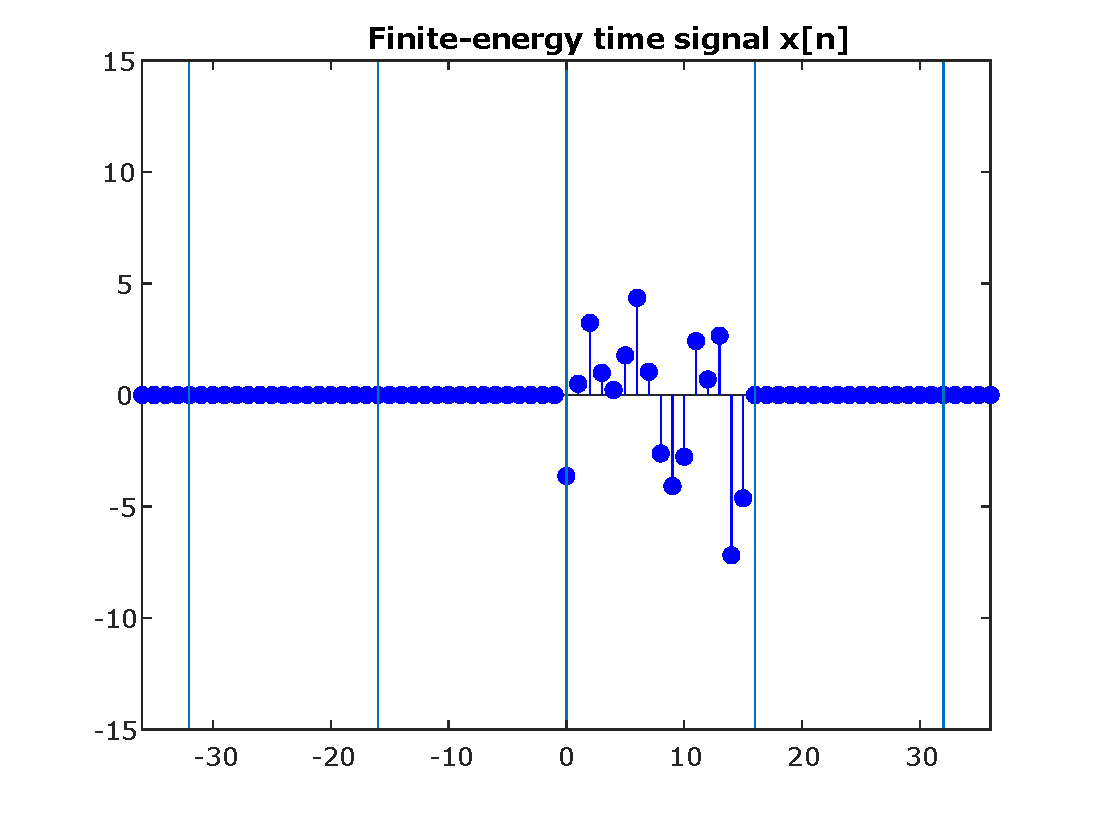
\includegraphics[width=\myimagewidth]{Pictures/FiniteEnergyTimeSignal.pdf}
\end{center}
&
\begin{center}

\underline{\textbf{Discrete Time Fourier Transform (DTFT)}}

\textcolor{gray}{\mportant{$\hat{x}(\theta)=\sum\limits_{n=-\infty}^\infty x[n]e^{-2\pi in\theta}$}}

\mportant{$X(\omega)=\sum\limits_{k=-\infty}^\infty x(k)e^{-j\omega k}$}

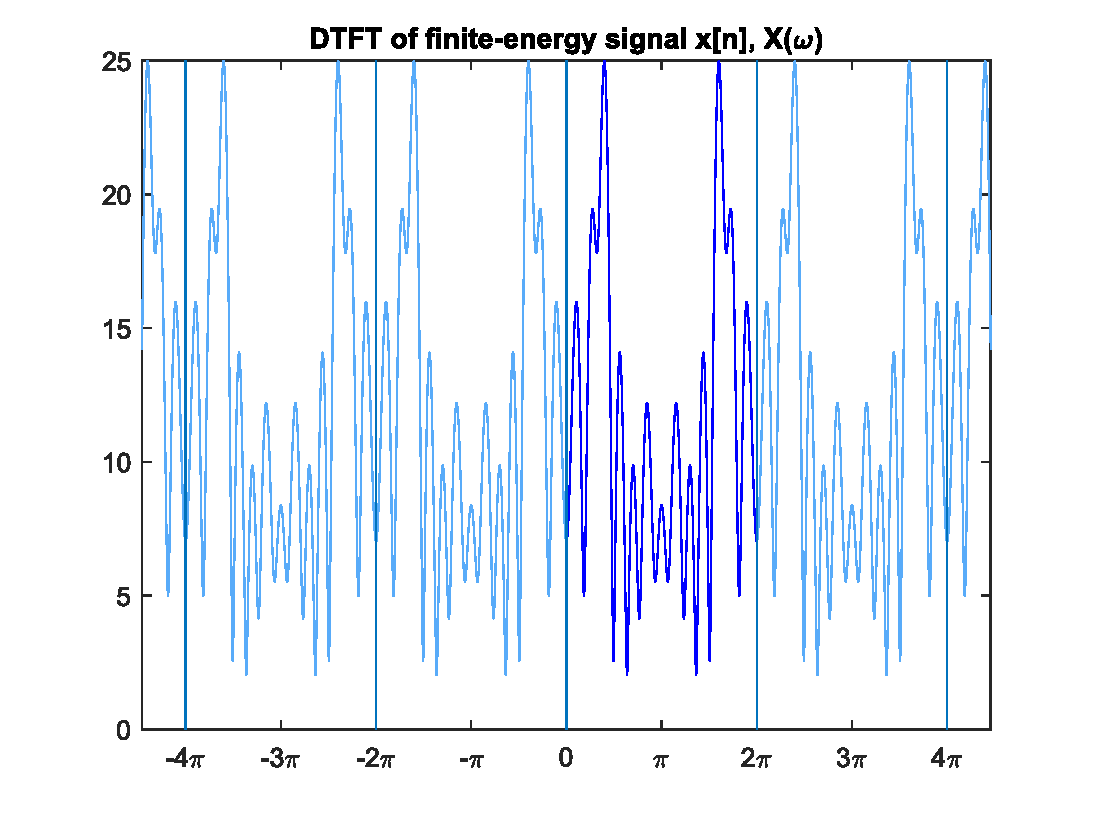
\includegraphics[width=\myimagewidth]{Pictures/DTFTFiniteEnergySignal.pdf}
\end{center}
&
\begin{center}
\underline{\textbf{Energy Spectral Density}}

\vspace{1.5cm}

\mportant{$S_x(\omega)=|X(\omega)|^2=\sum\limits_{\tau=-\infty}^\infty R_x(\tau)e^{-j\omega \tau}$}

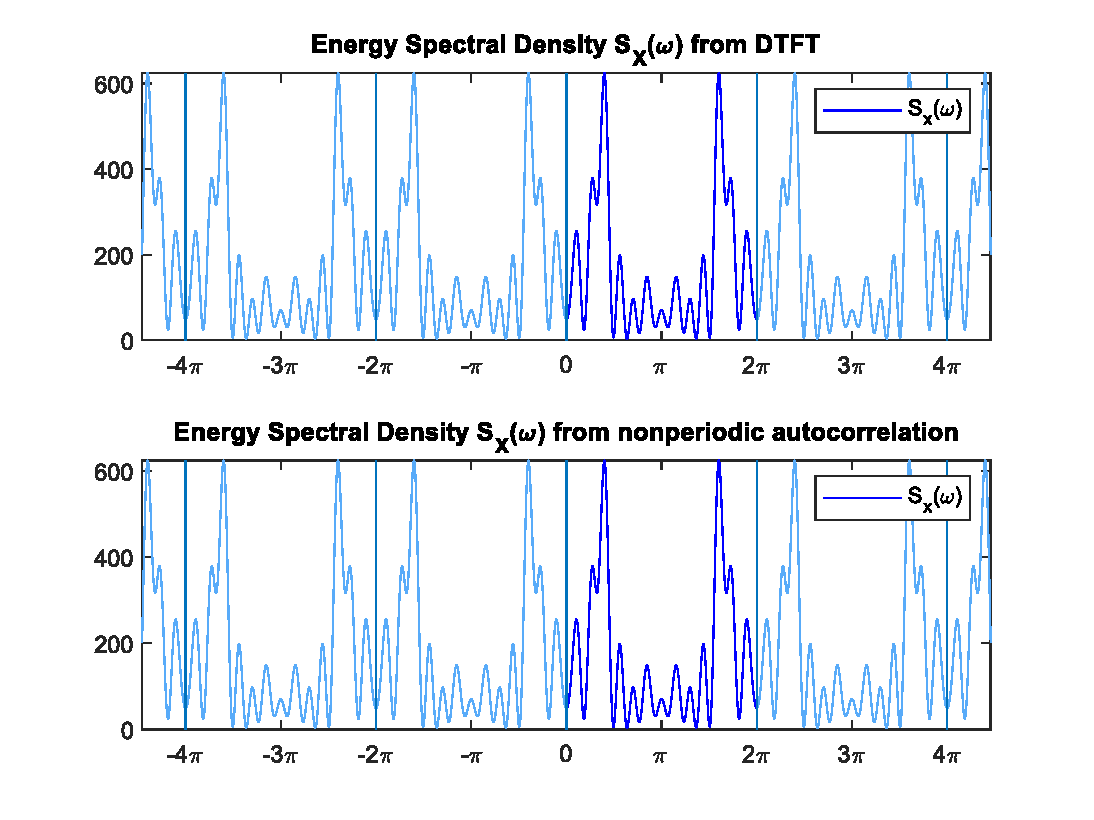
\includegraphics[width=\myimagewidth]{Pictures/EnergySpectralDensityFromNonPeriodicAutocorrelation.pdf}
\end{center}
&
\begin{center}
\underline{\textbf{Nonperiodic Autocorrelation}}

\vspace{1.5cm}

\mportant{$R_x(\tau)=\sum\limits_{k=-\infty}^\infty x(k)x(k-\tau)$}
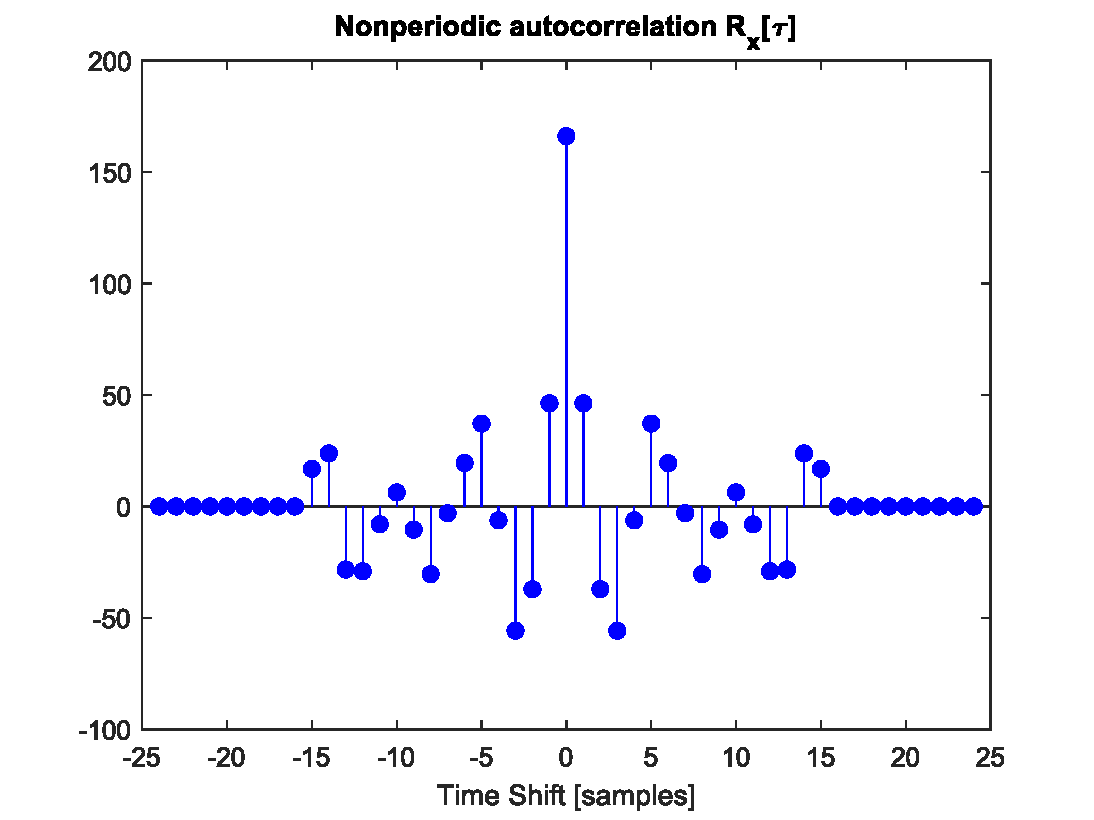
\includegraphics[width=\myimagewidth]{Pictures/NonPeriodicAutocorrelation.pdf}
\end{center}\\\hline

\begin{center}
\underline{\textbf{Periodic Time Domain Signal}}

\textcolor{gray}{\mportant{$x[n]=\frac{1}{N}\sum\limits_{k=0}^{N-1}\hat{x}[k]e^{2\pi in\frac{k}{N}}$}}

\mportant{$x(k)=\frac{1}{N}\sum\limits_{n=0}^{N-1}X(\omega_n)e^{j\omega_n k},\ \omega_n = 2\pi\frac{n}{N}$}

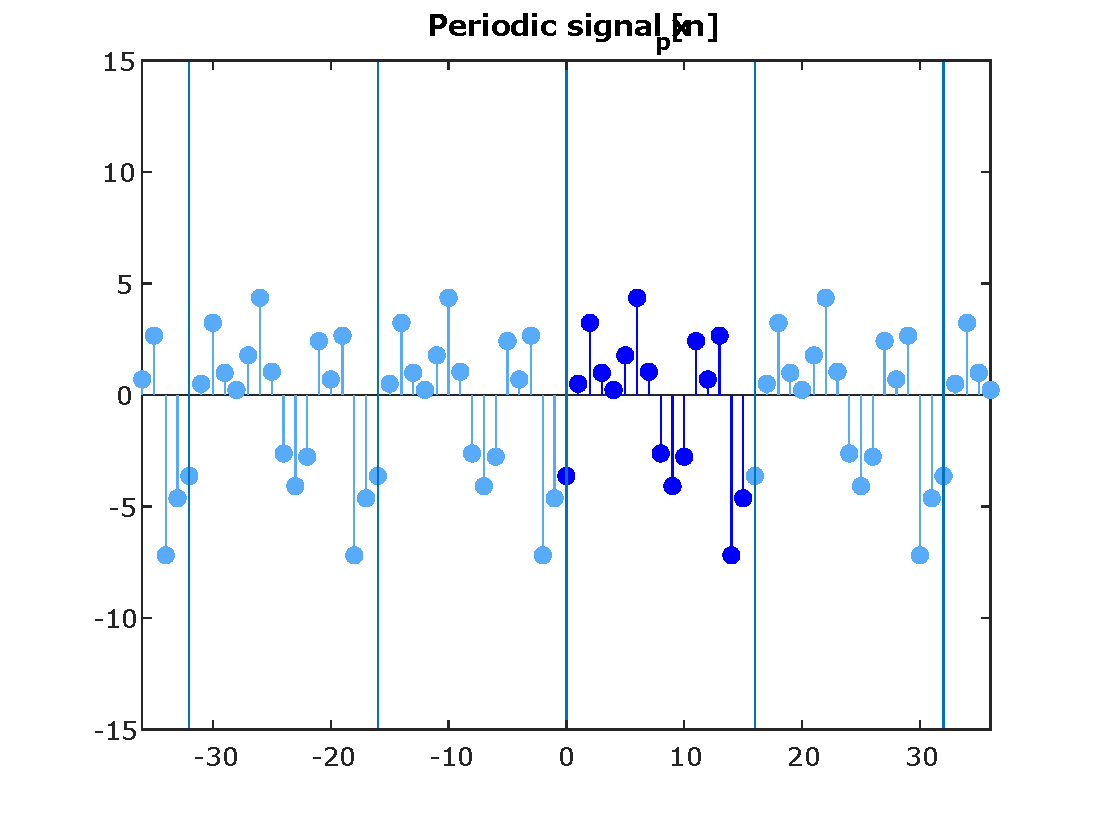
\includegraphics[width=\myimagewidth]{Pictures/PeriodicSignal.pdf}
\end{center}
&
\begin{center}
\underline{\textbf{Discrete Fourier Transform}}

\textcolor{gray}{\mportant{$\hat{x}[k]=\sum\limits_{n=0}^{N-1}x[n]e^{-2\pi ik\frac{n}{N}}$}}

\mportant{$X(\omega_n)=\sum\limits_{k=0}^{N-1}x(k)e^{-j\omega_n k},\ \omega_n=2\pi\frac{n}{N}$}
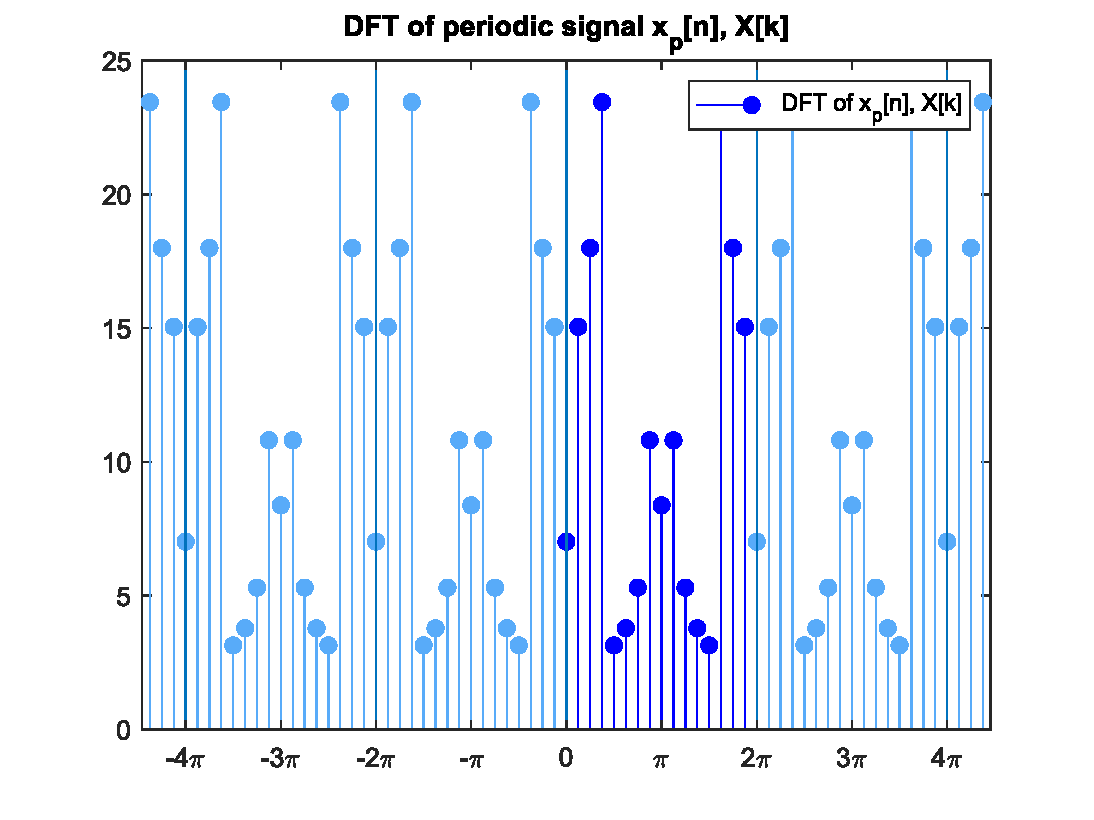
\includegraphics[width=\myimagewidth]{Pictures/DFTPeriodicSignal.pdf}
\end{center}
&
\begin{center}
\underline{\textbf{Power Spectral Density (PSD)}}

\vspace{1.5cm}

\mportant{$\phi(\omega_n)=\frac{1}{N}|X(\omega_n)|^2=\sum\limits_{\tau =0}^{N-1}R_x(\tau)e^{-j\omega_n\tau}$}

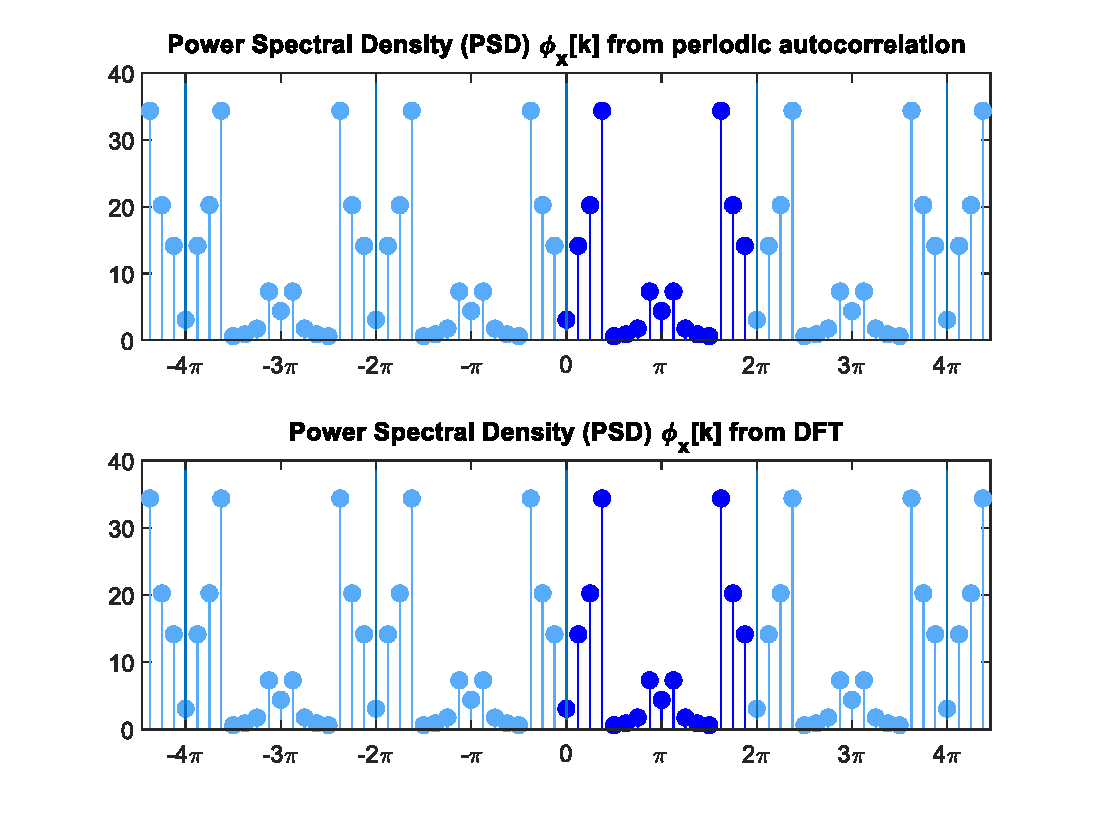
\includegraphics[width=\myimagewidth]{Pictures/PowerSpectralDensityFromDFT.pdf}
\end{center}
&
\begin{center}
\underline{\textbf{Periodic Autocorrelation}}

\vspace{1.5cm}

\mportant{$R_x(\tau)=\frac{1}{N}\sum\limits_{k=0}^{N-1}x(k)x(k-\tau)$}

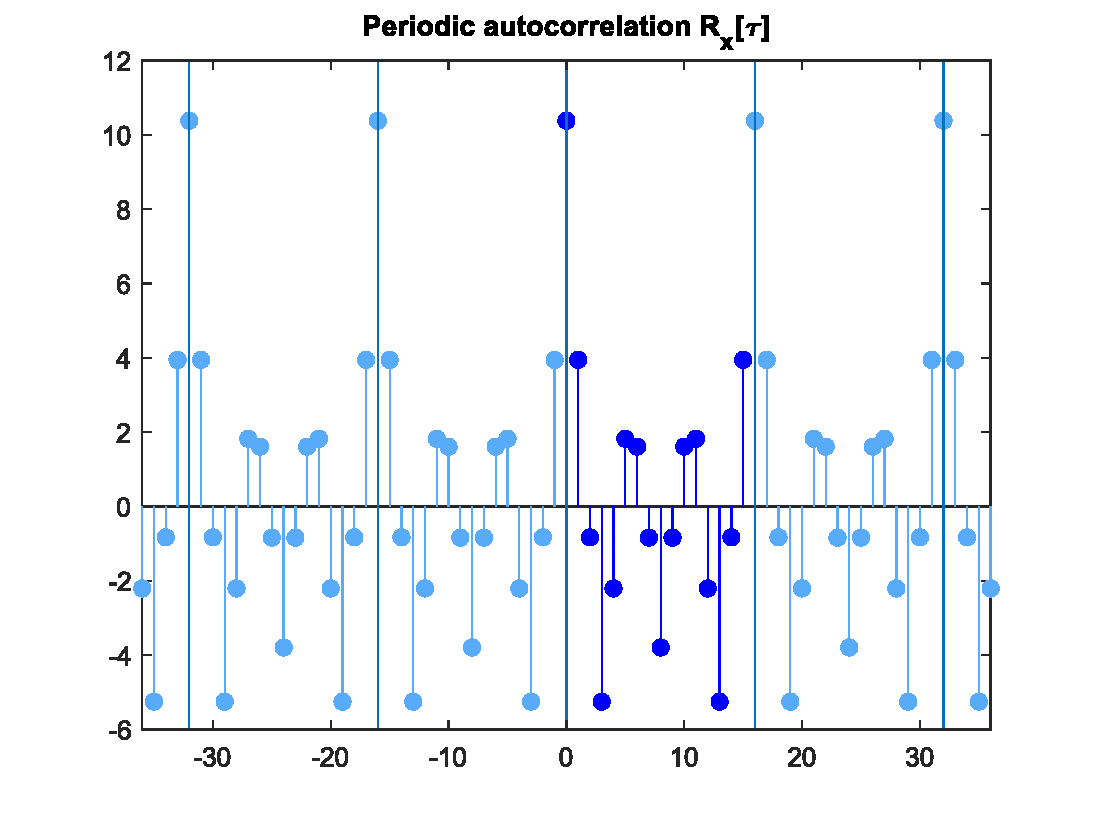
\includegraphics[width=\myimagewidth]{Pictures/PeriodicAutocorrelation.pdf}
\end{center}\\\hline
\end{tabular}
\normalsize

\newpage

\subsection{Transfer Function Estimation}

fill in coolness chart

\end{document}